% EPC flow charts
% Author: Fabian Schuh
\documentclass{minimal}

\usepackage{pgf}
\usepackage{tikz}
\usepackage[utf8]{inputenc}
\usetikzlibrary{arrows,automata}
\usetikzlibrary{positioning}


\tikzset{
    state/.style={
           rectangle,
           rounded corners,
           draw=black, very thick,
           minimum height=2em,
           inner sep=2pt,
           text centered,
           },
}

\begin{document}

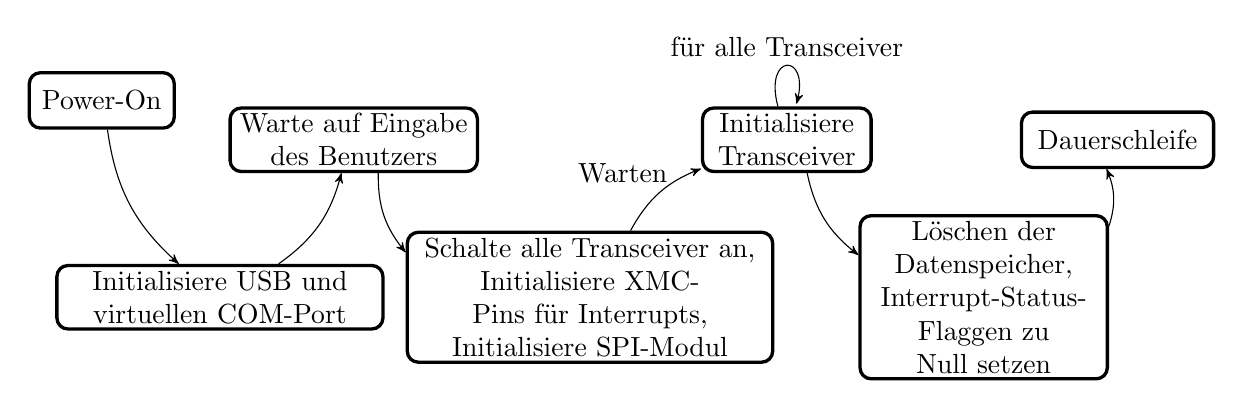
\begin{tikzpicture}[->,>=stealth']


 \node[state, text width=4cm] (Init1) 
 {Initialisiere USB und virtuellen COM-Port};


  \node[state,    	% layout (defined above)
  text width=1.7cm, 	% max text width
  yshift=2.5cm, 		% move 2cm in y
  left of=Init1, 	% Position is to the right of QUERY
  node distance=1.5cm, 	% distance to QUERY
  anchor=center] (Start) 	% posistion relative to the center of the 'box'
  {Power-On};

 \node[state,    	% layout (defined above)
  text width=3cm, 	% max text width
  yshift=2cm, 		% move 2cm in y
  right of=Init1, 	% Position is to the right of QUERY
  node distance=1.7cm, 	% distance to QUERY
  anchor=center] (Wait) 	% posistion relative to the center of the 'box'
 {Warte auf Eingabe des Benutzers};
 
 
  \node[state,    	% layout (defined above)
  text width=4.5cm, 	% max text width
  yshift=-2cm, 		% move 2cm in y
  right of=Wait, 	% Position is to the right of QUERY
  node distance=3cm, 	% distance to QUERY
  anchor=center] (Init2) 	% posistion relative to the center of the 'box'
  {Schalte alle Transceiver an,\\
  	Initialisiere XMC-Pins für Interrupts,\\
  	Initialisiere SPI-Modul};
  
%  warte, bestätige durch LED Blinken
 
  \node[state,    	% layout (defined above)
  text width=2cm, 	% max text width
  yshift=2cm, 		% move 2cm in y
  right of=Init2, 	% Position is to the right of QUERY
  node distance=2.5cm, 	% distance to QUERY
  anchor=center] (InitTDA) 	% posistion relative to the center of the 'box'
  {Initialisiere Transceiver};
  
   \node[state,    	% layout (defined above)
   text width=3cm, 	% max text width
   yshift=-2cm, 		% move 2cm in y
   right of=InitTDA, 	% Position is to the right of QUERY
   node distance=2.5cm, 	% distance to QUERY
   anchor=center] (setvariables) 	% posistion relative to the center of the 'box'
   {Löschen der Datenspeicher,\\
   	Interrupt-Status-Flaggen zu Null setzen};
 
 
 %ausgabe Warte auf Übertragungen
 
 
 
  \node[state,    	% layout (defined above)
  text width=2.3cm, 	% max text width
  yshift=2cm, 		% move 2cm in y
  right of=setvariables, 	% Position is to the right of QUERY
  node distance=1.7cm, 	% distance to QUERY
  anchor=center] (Dauer) 	% posistion relative to the center of the 'box'
  {Dauerschleife};
 
 
 
 
 
 

 % draw the paths and and print some Text below/above the graph

 
 \path 
 (Start)     	edge[bend right=20] node[anchor=south,above]{} (Init1)
 (Init1)     	edge[bend right=20] node[anchor=south,above]{} (Wait)
  (Wait)     	edge[bend right=20] node[anchor=south,above]{} (Init2)
   (Init2)     	edge[bend left=20] node[anchor=north,above]{Warten~~~~~~~~~} (InitTDA)
 (InitTDA)  	edge[loop above]    node[anchor=north,above]{für alle Transceiver} (InitTDA)
   (InitTDA)     	edge[bend right=20] node[anchor=south,above]{} (setvariables)   
   (setvariables)     	edge[bend right=20] node[anchor=south,above]{} (Dauer);
 
 

\end{tikzpicture}

































\end{document}